% Gemini theme
% https://github.com/anishathalye/gemini

\documentclass[final]{beamer}

% ====================
% Packages
% ====================

\usepackage[T1]{fontenc}
\usepackage{lmodern}
\usepackage[size=custom,width=96,height=48,scale=1]{beamerposter}
\usetheme{gemini}
\usecolortheme{gemini}
\usepackage{graphicx, amsmath, sidecap}
\usepackage{booktabs}
\usepackage{tikz}
\usepackage{pgfplots}

% ====================
% Lengths
% ====================

% If you have N columns, choose \sepwidth and \colwidth such that
% (N+1)*\sepwidth + N*\colwidth = \paperwidth
\newlength{\sepwidth}
\newlength{\colwidth}
\setlength{\sepwidth}{0.025\paperwidth}
\setlength{\colwidth}{0.3\paperwidth}

\newcommand{\separatorcolumn}{\begin{column}{\sepwidth}\end{column}}

% ====================
% Title
% ====================

\title{Tak: The Computational Toxicological Machine}

\author{Michael Chary, MD, PhD$^*$, Ed Boyer, MD, PhD, Michele Burns, MD MPH}

\institute[BCH Tox]{Division of Toxicology, Boston Children's Hospital}

% ====================
% Body
% ====================

\begin{document}

\begin{frame}[t]
\begin{columns}[t]
\separatorcolumn

\begin{column}{\colwidth}

  \begin{block}{Introduction}

    There is simply too much to think about. 

    \begin{figure}
   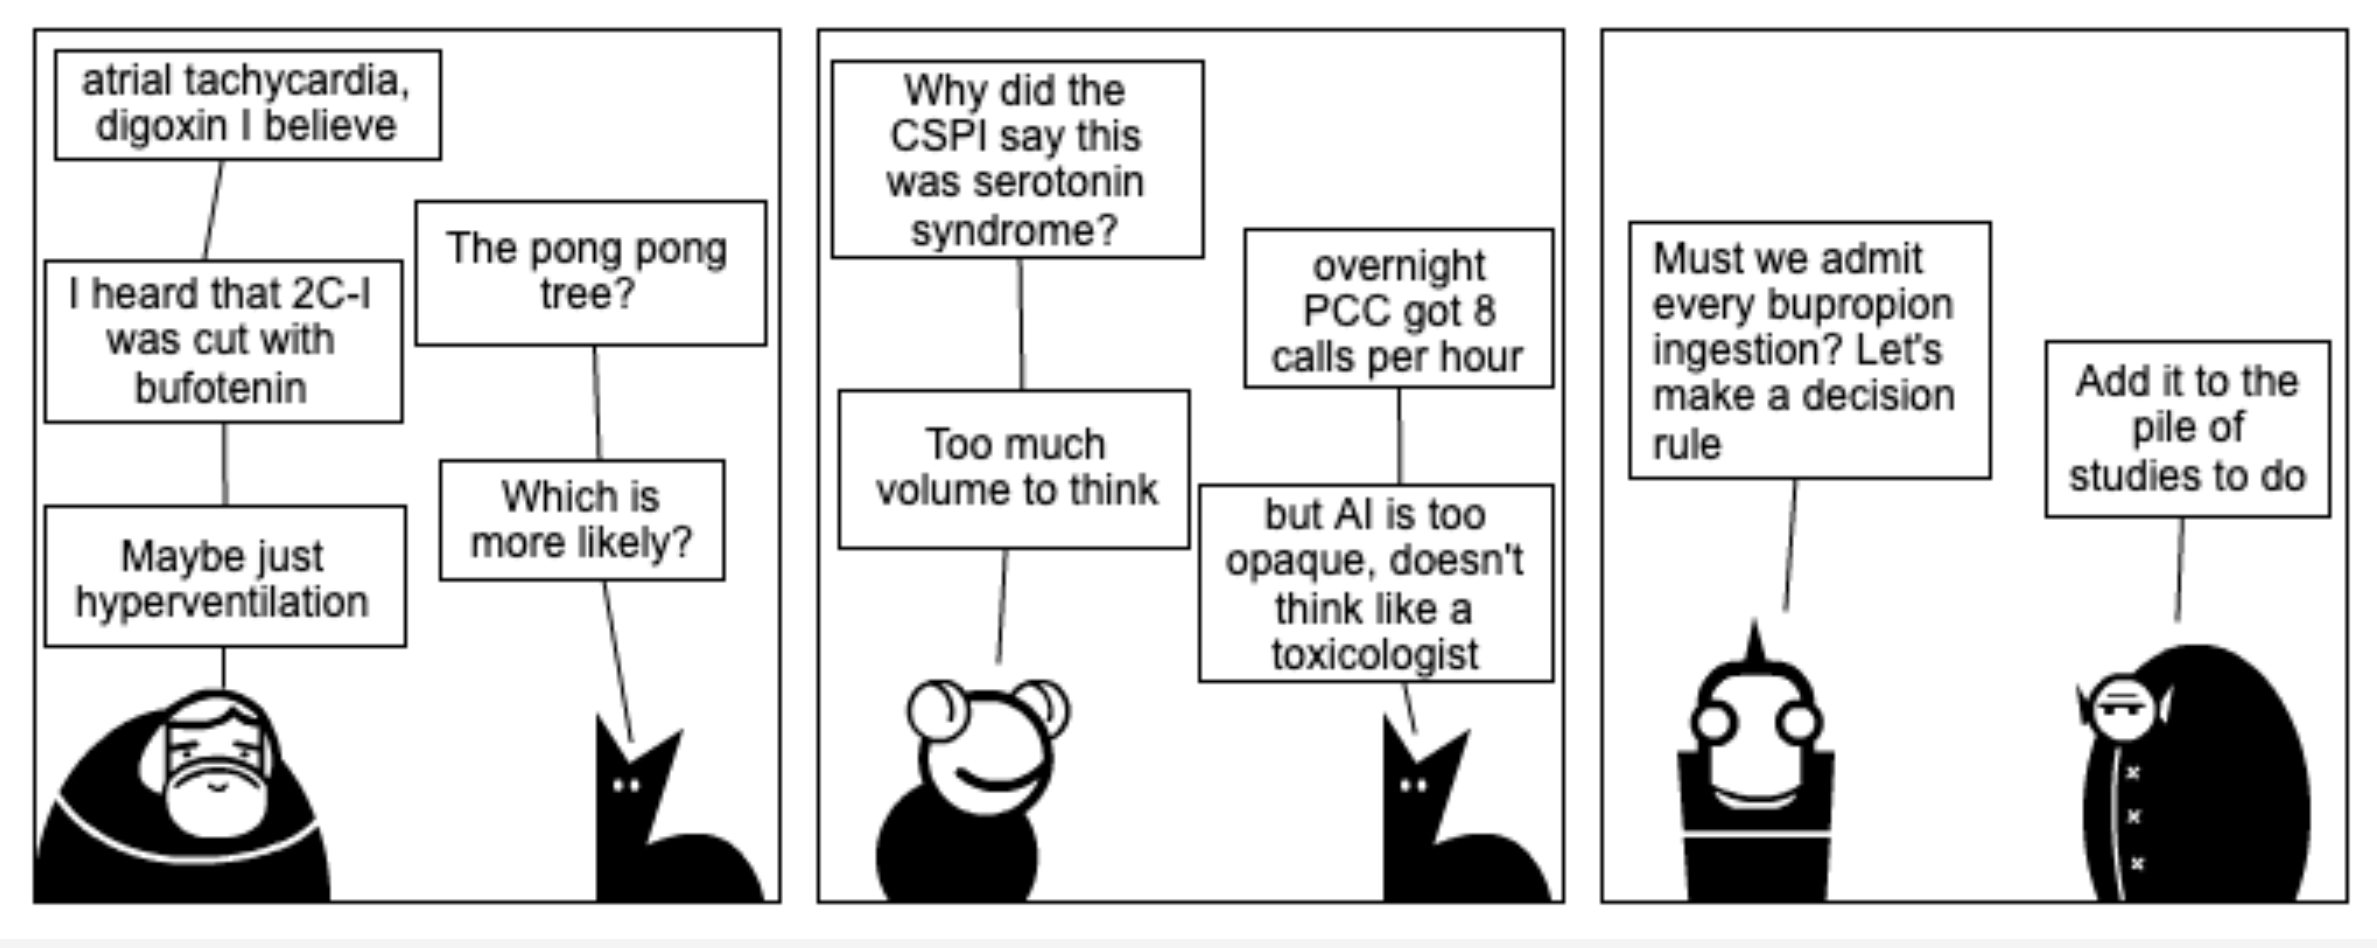
\includegraphics[scale=0.65]{./acmt-intro.png}
   \end{figure}

     \begin{itemize}
      \item[] Clinical, scientific knowledge are too vast for one person or team to master.
      \item[] If only we could  \textbf{combine machine speed with human intuition}\ldots  
    \end{itemize}
  \end{block}


  \begin{alertblock}{Probabilistic Logic}
   
         If someone is not tachycardic, s/he is not anticholinergic. 
       
      $NOT \textrm{tachycardic}\left(x\right) \rightarrow NOT \textrm{anticholinergic}\left(x\right)$
      
      \vspace{1em}
      If someone is tachycardic, s/he is $x$ times more likely to to be anticholinergic or sympathomimetic then cholinergic. 
      
       \begin{align*}
                 & 	x\;  \textrm{tachycardic}\left(x\right) \rightarrow \textrm{anticholinergic}\left(x\right)\\
            	& x \; \textrm{tachycardic}\left(x\right) \rightarrow \textrm{sympathomimetic}\left(x\right)\\
            	& 0.1x \; \textrm{tachycardic}\left(x\right) \rightarrow \textrm{cholinergic}\left(x\right)\\
      \end{align*}

  \end{alertblock}

\end{column}

\separatorcolumn

\begin{column}{\colwidth}

  \begin{block}{Approach}

    Our approach is to distill the diagnosis of toxidromes into probabilistic (fuzzy) rules and then evaluate the performance of those rules against human raters. We use synthetic patients as our test data set. Objectives:


    \begin{itemize}
      \item \textbf{Develop} artificial intelligence that diagnoses toxidrome from simple presentations (as might be given in an initial call)
      \item \textbf{Compare} AI to human performance
    \end{itemize}
  \end{block}

  \begin{block}{Results}

    
     \begin{figure}
     \begin{minipage}{0.6\colwidth}
         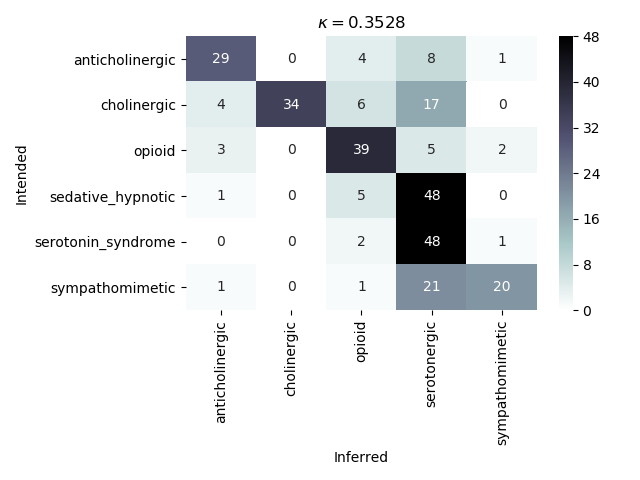
\includegraphics{./inferred-intended-overall.png}
 \end{minipage}\begin{minipage}{0.35\colwidth}
  
      \caption{\textbf{Confusion matrix between intended and predicted diagnoses.} Axis shows rater. Axis label shows mostly likely toxidrome. Number and color in each grid of heat map show the number of diagnoses. $\kappa$ denotes Cohen's $\kappa$.}
      \end{minipage}
     
    \end{figure}

  \end{block}

  \begin{block}{Nam cursus consequat egestas}

    Nulla eget sem quam. Ut aliquam volutpat nisi vestibulum convallis. Nunc a
    lectus et eros facilisis hendrerit eu non urna. Interdum et malesuada fames
    ac ante \textit{ipsum primis} in faucibus. Etiam sit amet velit eget sem
    euismod tristique. Praesent enim erat, porta vel mattis sed, pharetra sed
    ipsum. Morbi commodo condimentum massa, \textit{tempus venenatis} massa
    hendrerit quis. Maecenas sed porta est. Praesent mollis interdum lectus,
    sit amet sollicitudin risus tincidunt non.

    Etiam sit amet tempus lorem, aliquet condimentum velit. Donec et nibh
    consequat, sagittis ex eget, dictum orci. Etiam quis semper ante. Ut eu
    mauris purus. Proin nec consectetur ligula. Mauris pretium molestie
    ullamcorper. Integer nisi neque, aliquet et odio non, sagittis porta justo.

    \begin{itemize}
      \item \textbf{Sed consequat} id ante vel efficitur. Praesent congue massa
        sed est scelerisque, elementum mollis augue iaculis.
        \begin{itemize}
          \item In sed est finibus, vulputate
            nunc gravida, pulvinar lorem. In maximus nunc dolor, sed auctor eros
            porttitor quis.
          \item Fusce ornare dignissim nisi. Nam sit amet risus vel lacus
            tempor tincidunt eu a arcu.
          \item Donec rhoncus vestibulum erat, quis aliquam leo
            gravida egestas.
        \end{itemize}
      \item \textbf{Sed luctus, elit sit amet} dictum maximus, diam dolor
        faucibus purus, sed lobortis justo erat id turpis.
      \item \textbf{Pellentesque facilisis dolor in leo} bibendum congue.
        Maecenas congue finibus justo, vitae eleifend urna facilisis at.
    \end{itemize}

  \end{block}

\end{column}

\separatorcolumn

\begin{column}{\colwidth}

  \begin{block}{Comparison with Human Raters}
     
     
     \begin{figure}
     \centering
     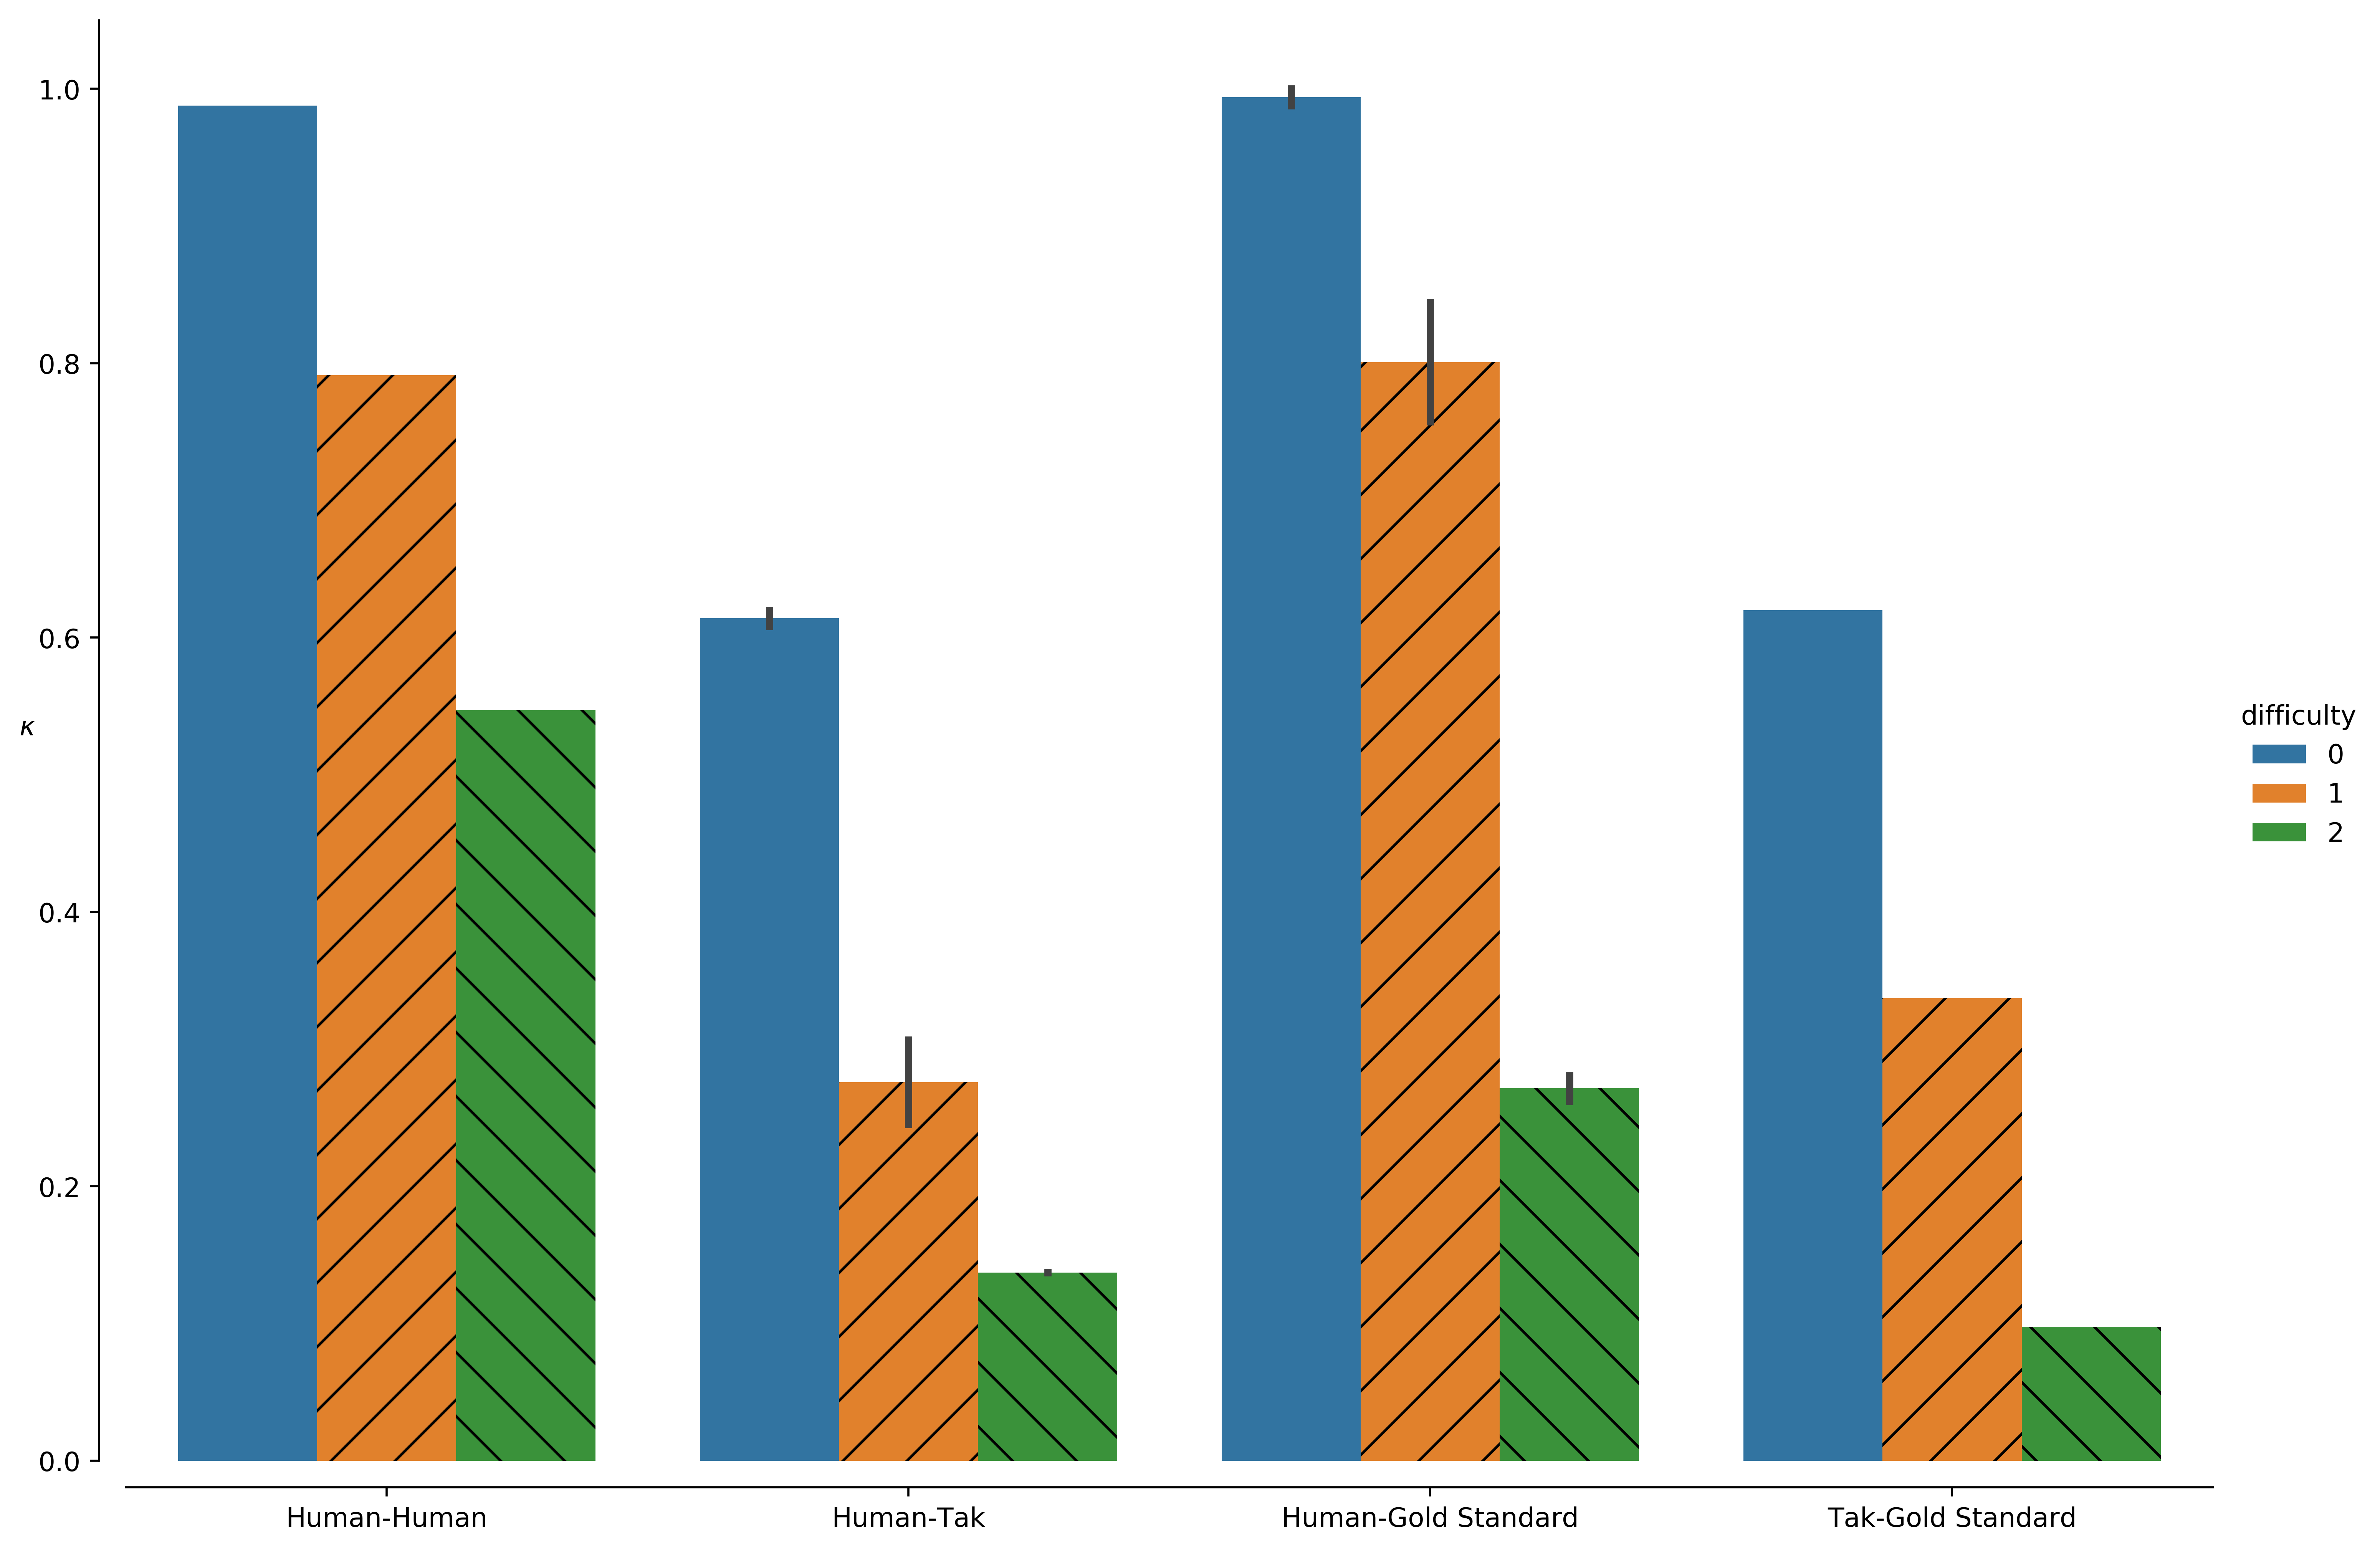
\includegraphics[scale=0.8]{combined-kappas.png}
     \caption{\textbf{Human and Computer Agreement} Y-axis denotes Cohen's $\kappa$. X-axis denotes pair; Human raters, Intended (actual) labels, and Inferred (Tak) labels. Hue indicates difficulty of presentation. Refers to number of noncanonical symptoms in presentation.}
     \end{figure}

  \end{block}

  \begin{block}{Conclusions}

    Class aptent taciti sociosqu ad litora torquent per conubia nostra, per
    inceptos himenaeos. Phasellus libero enim, gravida sed erat sit amet,
    scelerisque congue diam. Fusce dapibus dui ut augue pulvinar iaculis.


    Nulla varius finibus volutpat. Mauris molestie lorem tincidunt, iaculis
    libero at, gravida ante. Phasellus at felis eu neque suscipit suscipit.
    Integer ullamcorper, dui nec pretium ornare, urna dolor consequat libero,
    in feugiat elit lorem euismod lacus. Pellentesque sit amet dolor mollis,
    auctor urna non, tempus sem.

  \end{block}

\end{column}

\separatorcolumn
\end{columns}
\end{frame}

\end{document}
